% ============================================================
% 3.2.3.3 Inflation and Deflation
% AQA AS Economics
% Sources: output/authoritative/as_syllabus.json (3.2.3.3)
%          output/authoritative/sow.json (as > 3.2 > 3.2.3)
% Suggested timing: 5 hours
% ============================================================

\documentclass[16pt,aspectratio=169]{beamer}
\usetheme{Madrid}
\usecolortheme{default}

\usepackage{graphicx}
\graphicspath{{../../../../../assets/images/}{./figures/}}
\usepackage{booktabs}
\usepackage{tikz}
\usepackage{pgfplots}
\pgfplotsset{compat=1.18}
\RequirePackage{tcolorbox}
\tcbuselibrary{skins}

% Key Point — yellow; for the single most important idea on a slide
\newtcolorbox{keypoint}{
    enhanced,
    colback=yellow!12,
    colframe=yellow!60!black,
    fonttitle=\bfseries,
    title=Key Point,
    arc=2pt,
    boxrule=0.8pt,
}

% Formula — blue; for named equations and their variable key
\newtcolorbox{formula}[1][Formula]{
    enhanced,
    colback=blue!5,
    colframe=blue!45!black,
    fonttitle=\bfseries,
    title=#1,
    arc=2pt,
    boxrule=0.8pt,
}

% Example Question — teal; for exam-style questions posed to students
\newtcolorbox{examplequestion}[1][Example Question]{
    enhanced,
    colback=teal!6,
    colframe=teal!55!black,
    fonttitle=\bfseries,
    title=#1,
    arc=2pt,
    boxrule=0.8pt,
}

% Example Solution — green; always follows an examplequestion block
\newtcolorbox{examplesolution}[1][Solution]{
    enhanced,
    colback=green!6,
    colframe=green!45!black,
    fonttitle=\bfseries,
    title=#1,
    arc=2pt,
    boxrule=0.8pt,
}

% ---- Worksheet environments --------------------------------

% Scenario — blue; for group discussion prompts on worksheets
% Usage: \begin{scenario}{Scenario 1: Title with commas, fine} ... \end{scenario}
\newtcolorbox{scenario}[1]{
    enhanced,
    colback=blue!5,
    colframe=blue!45!black,
    fonttitle=\bfseries,
    title={#1},
    arc=2pt,
    boxrule=0.8pt,
}

% Instructions — blue; for worksheet-level instruction blocks
\newtcolorbox{instructions}{
    enhanced,
    colback=blue!5,
    colframe=blue!45!black,
    fonttitle=\bfseries,
    title=Instructions,
    arc=2pt,
    boxrule=0.8pt,
}

% Extract — grey; for data response source material
% Usage: \begin{extract}{Source: Author, Year} ... \end{extract}
\newtcolorbox{extract}[1]{
    enhanced,
    colback=gray!8,
    colframe=gray!50,
    fonttitle=\bfseries,
    title={#1},
    arc=2pt,
    boxrule=0.8pt,
}


\title{Inflation and Deflation}
\subtitle{3.2.3.3 | AQA AS Economics}
\author{Dr Jac Thomas}
\date{\today}

\begin{document}

% ---- Title -------------------------------------------------
\begin{frame}
    \titlepage
\end{frame}

% ---- Learning Objectives -----------------------------------
\begin{frame}{Learning Objectives}
    \textbf{To be able to\ldots}
    \begin{itemize}
        \item Define inflation, deflation, and disinflation, and distinguish clearly between them
        \item Explain demand-pull and cost-push causes of inflation using AD/AS diagrams
        \item Analyse how changes in world commodity prices affect domestic inflation
        \item Explain how economic changes in other countries affect UK inflation
        \item Understand what ``deflationary policies'' means and why it does not mean causing deflation
        \item Apply index-number skills to measure and interpret price changes
    \end{itemize}
\end{frame}

% ---- What is Inflation? ------------------------------------
\begin{frame}{What is Inflation?}
    \begin{definition}
        \textbf{Inflation} is a sustained rise in the general price level of goods and services in an economy over time.
    \end{definition}

    \vspace{0.8em}
    \textbf{Why does it matter?}
    \begin{itemize}
        \item Erodes the purchasing power of money --- real incomes fall if wages do not keep up
        \item Creates uncertainty: firms find it harder to plan investment
        \item May harm export competitiveness if domestic prices rise faster than abroad
        \item Redistributes income from savers to borrowers (real value of debt falls)
        \item The Bank of England's target is \textbf{2\% CPI inflation} --- a key macroeconomic policy objective
    \end{itemize}
\end{frame}

\begin{frame}{What is Inflation? --- Measurement}
    \begin{keypoint}
        Inflation is measured using price indices such as the Consumer Prices Index (CPI). A stable, low rate of inflation is generally preferred to zero inflation or deflation.
    \end{keypoint}
\end{frame}

% ---- Measuring Inflation: CPI ------------------------------
\begin{frame}{Measuring Inflation: The Consumer Prices Index (CPI)}
    The CPI tracks changes in the price of a \textbf{weighted basket of goods and services} representing the spending of a typical UK household.

    \vspace{0.6em}
    \textbf{How it works:}
    \begin{enumerate}
        \item A basket of around 700 items is selected (updated annually)
        \item Each item is given a \textbf{weight} proportional to its share of household spending
        \item Prices are collected monthly from thousands of outlets
        \item A \textbf{weighted average} price index is calculated
    \end{enumerate}

    \vspace{0.5em}
    \begin{columns}
        \begin{column}{0.47\textwidth}
            \textbf{CPI (used for Bank of England target):}
            \begin{itemize}
                \item Excludes housing costs
                \item Internationally comparable
            \end{itemize}
        \end{column}
        \begin{column}{0.47\textwidth}
            \textbf{RPI (older measure):}
            \begin{itemize}
                \item Includes mortgage interest and council tax
                \item Higher than CPI --- used for some index-linked contracts
            \end{itemize}
        \end{column}
    \end{columns}
\end{frame}

% ---- Deflation and Disinflation ----------------------------
\begin{frame}{Deflation and Disinflation: A Critical Distinction}
    \begin{columns}
        \begin{column}{0.47\textwidth}
            \begin{definition}
                \textbf{Deflation} exists when the \textit{price level is falling} --- the rate of inflation is negative.
            \end{definition}
            \vspace{0.4em}
            \textbf{Why deflation is harmful:}
            \begin{itemize}
                \item Consumers delay purchases expecting prices to fall further
                \item Firms cut output and employment
                \item Real value of debt rises --- firms and households struggle to repay
                \item Japan's ``Lost Decade'': persistent deflation trapped the economy
            \end{itemize}
        \end{column}
        \begin{column}{0.47\textwidth}
            \begin{definition}
                \textbf{Disinflation} is when the \textit{rate of inflation is falling} --- prices are still rising, but more slowly.
            \end{definition}
            \vspace{0.4em}
            \begin{example}
                If CPI inflation falls from 6\% to 2\%, this is \textbf{disinflation} --- not deflation. The price level is still rising; it is just rising more slowly.
            \end{example}
            \vspace{0.3em}
            \alert{Common error:} Disinflation $\neq$ Deflation. Disinflation means the rate of price increase slows --- prices are not falling.
        \end{column}
    \end{columns}
\end{frame}

% ---- Deflationary Policies ---------------------------------
\begin{frame}{Deflationary Policies: An Important Distinction}
    \begin{keypoint}
        ``Deflationary policies'' are policies to \textbf{reduce aggregate demand} and slow the rate of inflation. They do \textbf{not} necessarily cause the price level to fall (deflation).
    \end{keypoint}

    \vspace{0.7em}
    \textbf{Examples of deflationary policies:}
    \begin{itemize}
        \item Raising interest rates (monetary policy) --- reduces consumer borrowing and investment
        \item Cutting government spending or raising taxes (fiscal policy) --- reduces AD
    \end{itemize}

    \vspace{0.5em}
    \textbf{The goal is to move the economy from, say, 7\% inflation back toward 2\% --- not to make prices fall outright.}
\end{frame}

\begin{frame}{Deflationary Policies: Real-World Example}
    \begin{example}
        In 2022--23, the Bank of England raised interest rates from 0.1\% to 5.25\%. This was a \textbf{deflationary policy} (intended to reduce inflation from 11\%). CPI inflation fell to around 2\% by mid-2024 --- this is \textbf{disinflation}, not deflation.
    \end{example}
\end{frame}

% ---- Demand-Pull Inflation ---------------------------------
\begin{frame}{Demand-Pull Inflation --- Definition}
    \begin{definition}
        \textbf{Demand-pull inflation} occurs when aggregate demand rises faster than the economy's productive capacity, pulling the price level upward.
    \end{definition}
\end{frame}

% SRAS:  P = Y
% LRAS:  Y = 7  (= Yf)
% AD1:   P = 8 - Y   =>  E1: Y=4, P=4
% AD2:   P = 16 - Y  =>  E2: Y=8, P=8  (positive output gap: Y2 > Yf)
% xmax = 13  (>= 8 * 1.25 = 10, plus label room)
% ymax = 11
\begin{frame}{Demand-Pull Inflation --- AD/AS Diagram}
    \begin{columns}
        \begin{column}{0.55\textwidth}
            \begin{center}
                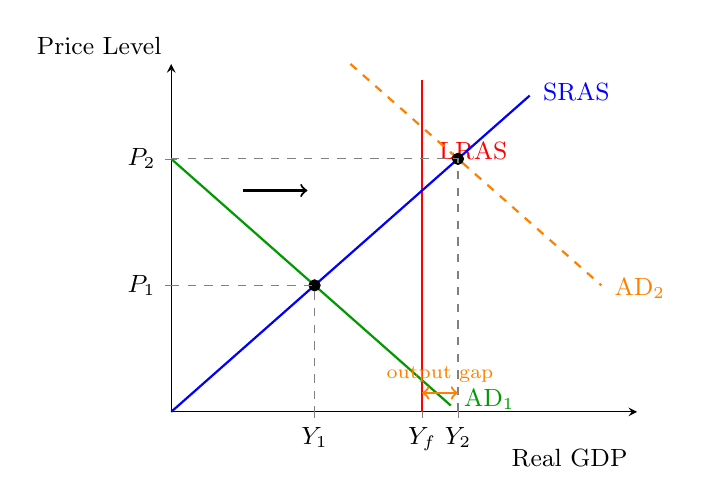
\begin{tikzpicture}
                    \begin{axis}[
                        axis lines = middle,
                        xmin=0, xmax=13, ymin=0, ymax=11,
                        xtick={4, 7, 8},
                        xticklabels={$Y_1$, $Y_f$, $Y_2$},
                        ytick={4, 8},
                        yticklabels={$P_1$, $P_2$},
                        width=7.5cm, height=6cm,
                        xlabel={Real GDP},
                        ylabel={Price Level},
                        xlabel style={at={(axis description cs:1,0)}, anchor=north east, yshift=-10pt, font=\small},
                        ylabel style={at={(axis description cs:0,1)}, anchor=south east, font=\small},
                        tick label style={font=\small},
                        clip=false,
                    ]
                    % LRAS at Yf=7
                    \addplot[red, thick] coordinates {(7,0) (7,10.5)};
                    \node[red, font=\small, anchor=west] at (axis cs: 7.2, 8.25) {LRAS};
                    % SRAS: P = Y; label beyond right end at (9.8, 9.8)
                    \addplot[blue, thick, domain=0:10] {x};
                    \node[blue, font=\small, anchor=west] at (axis cs: 10.1, 10.1) {SRAS};
                    % AD1: P = 8 - Y; domain [0,8]; label near bottom-right
                    \addplot[green!60!black, thick, domain=0:7.8] {8 - x};
                    \node[green!60!black, font=\small, anchor=west] at (axis cs: 7.9, 0.4) {AD$_1$};
                    % AD2: P = 16 - Y; domain [5, 12]; label near bottom-right
                    \addplot[orange, thick, dashed, domain=5:12] {16 - x};
                    \node[orange, font=\small, anchor=west] at (axis cs: 12.1, 3.9) {AD$_2$};
                    % AD shift arrow (rightward, at mid-height between curves)
                    \draw[->, thick, black] (axis cs: 2, 7) -- (axis cs: 3.8, 7);
                    % Equilibrium points
                    \coordinate (E1) at (axis cs: 4, 4);
                    \coordinate (E2) at (axis cs: 8, 8);
                    \filldraw (E1) circle (2pt);
                    \filldraw (E2) circle (2pt);
                    % Dashed reference lines from E1
                    \draw[dashed, gray] (axis cs: 0, 4) -- (E1) -- (axis cs: 4, 0);
                    % Dashed reference lines from E2
                    \draw[dashed, gray] (axis cs: 0, 8) -- (E2) -- (axis cs: 8, 0);
                    % Positive output gap arrow
                    \draw[<->, thick, orange]
                        (axis cs: 7, 0.6) -- node[above, font=\scriptsize]{output gap} (axis cs: 8, 0.6);
                    \end{axis}
                \end{tikzpicture}
            \end{center}
        \end{column}
        \begin{column}{0.42\textwidth}
            \textbf{Causes (anything that raises AD):}
            \begin{itemize}\setlength\itemsep{0.2em}
                \item \small Cut in interest rates $\Rightarrow$ more borrowing
                \item \small Rise in consumer confidence
                \item \small Expansionary fiscal policy (higher G or lower T)
                \item \small Boom in trading partners $\Rightarrow$ higher exports
            \end{itemize}
            \vspace{0.3em}
            \textbf{Result:} $P_1 \to P_2$; positive output gap ($Y_2 > Y_f$)
        \end{column}
    \end{columns}
\end{frame}

% ---- Cost-Push Inflation -----------------------------------
\begin{frame}{Cost-Push Inflation --- Definition}
    \begin{definition}
        \textbf{Cost-push inflation} occurs when rising production costs shift SRAS leftward, raising the price level while reducing output.
    \end{definition}
\end{frame}

% SRAS1: P = Y
% SRAS2: P = Y + 4  (parallel shift; vertical intercept rises by 4)
% LRAS:  Y = 7  (= Yf)
% AD:    P = 10 - Y
% E1: SRAS1 ∩ AD:  Y = 10-Y  =>  Y=5, P=5
% E2: SRAS2 ∩ AD:  Y+4 = 10-Y  =>  Y=3, P=7
% xmax = 11  (>= 7 * 1.25)
% ymax = 11
\begin{frame}{Cost-Push Inflation --- AD/AS Diagram}
    \begin{columns}
        \begin{column}{0.55\textwidth}
            \begin{center}
                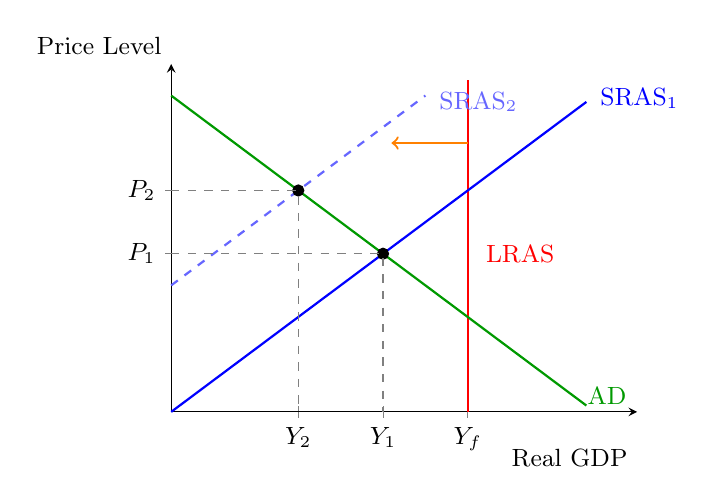
\begin{tikzpicture}
                    \begin{axis}[
                        axis lines = middle,
                        xmin=0, xmax=11, ymin=0, ymax=11,
                        xtick={3, 5, 7},
                        xticklabels={$Y_2$, $Y_1$, $Y_f$},
                        ytick={5, 7},
                        yticklabels={$P_1$, $P_2$},
                        width=7.5cm, height=6cm,
                        xlabel={Real GDP},
                        ylabel={Price Level},
                        xlabel style={at={(axis description cs:1,0)}, anchor=north east, yshift=-10pt, font=\small},
                        ylabel style={at={(axis description cs:0,1)}, anchor=south east, font=\small},
                        tick label style={font=\small},
                        clip=false,
                    ]
                    % LRAS at Yf=7
                    \addplot[red, thick] coordinates {(7,0) (7,10.5)};
                    \node[red, font=\small, anchor=west] at (axis cs: 7.2, 5.0) {LRAS};
                    % SRAS1: P = Y; label beyond rightmost point
                    \addplot[blue, thick, domain=0:9.8] {x};
                    \node[blue, font=\small, anchor=west] at (axis cs: 9.9, 9.9) {SRAS$_1$};
                    % SRAS2: P = Y + 4; domain [0, 6]; label beyond endpoint
                    \addplot[blue!60, thick, dashed, domain=0:6] {x + 4};
                    \node[blue!60, font=\small, anchor=west] at (axis cs: 6.1, 9.8) {SRAS$_2$};
                    % AD: P = 10 - Y; domain [0, 10]
                    \addplot[green!60!black, thick, domain=0:9.8] {10 - x};
                    \node[green!60!black, font=\small, anchor=west] at (axis cs: 9.6, 0.5) {AD};
                    % Leftward shift arrow (SRAS shifts left = costs rise)
                    \draw[->, thick, orange] (axis cs: 7.0, 8.5) -- (axis cs: 5.2, 8.5);
                    % Equilibrium points
                    \coordinate (E1) at (axis cs: 5, 5);
                    \coordinate (E2) at (axis cs: 3, 7);
                    \filldraw (E1) circle (2pt);
                    \filldraw (E2) circle (2pt);
                    % Dashed reference lines from E1
                    \draw[dashed, gray] (axis cs: 0, 5) -- (E1) -- (axis cs: 5, 0);
                    % Dashed reference lines from E2
                    \draw[dashed, gray] (axis cs: 0, 7) -- (E2) -- (axis cs: 3, 0);
                    \end{axis}
                \end{tikzpicture}
            \end{center}
        \end{column}
        \begin{column}{0.42\textwidth}
            \textbf{Causes (anything that raises input costs):}
            \begin{itemize}\setlength\itemsep{0.2em}
                \item \small Rise in oil or energy prices
                \item \small Rise in wages above productivity growth
                \item \small Depreciation of exchange rate (imports dearer)
                \item \small Rise in raw material prices globally
            \end{itemize}
            \vspace{0.3em}
            \textbf{Result:} $P_1 \to P_2$ (prices rise); $Y_1 \to Y_2$ (output falls) --- \textbf{stagflation}
        \end{column}
    \end{columns}
\end{frame}

% ---- Quantitative Skills -----------------------------------
\begin{frame}{Quantitative Skills: Index Numbers and the CPI}
    \textbf{A price index compares today's price level with a base year (= 100).}

    \vspace{0.3em}
    \[
        \text{Price Index} = \frac{\text{Price in current year}}{\text{Price in base year}} \times 100
        \qquad
        \text{Inflation rate} = \frac{\text{CPI}_t - \text{CPI}_{t-1}}{\text{CPI}_{t-1}} \times 100
    \]

    \vspace{0.5em}
    \begin{examplequestion}
        A simplified CPI uses two goods: food (weight 60\%) and transport (weight 40\%). Food prices rise from £5.00 to £5.50; transport prices rise from £10.00 to £10.20. Calculate the overall CPI and the inflation rate.
    \end{examplequestion}
\end{frame}

\begin{frame}{Quantitative Skills: Worked Solution}
    \begin{examplesolution}
        Food index: $\dfrac{5.50}{5.00} \times 100 = 110$ \quad Transport index: $\dfrac{10.20}{10.00} \times 100 = 102$

        \vspace{0.3em}
        CPI $= 0.60 \times 110 + 0.40 \times 102 = 66.0 + 40.8 = \mathbf{106.8}$

        \vspace{0.3em}
        Inflation rate $= \dfrac{106.8 - 100}{100} \times 100 = \mathbf{6.8\%}$
    \end{examplesolution}
\end{frame}

% ---- World Commodity Prices --------------------------------
\begin{frame}{World Commodity Prices and UK Inflation}
    \textbf{Commodity prices} (oil, gas, metals, food crops) are set in global markets. Changes transmit directly into UK inflation.

    \vspace{0.5em}
    \begin{table}
        \centering
        \small
        \renewcommand{\arraystretch}{1.15}
        \begin{tabular}{@{}p{4.2cm}p{3.5cm}p{4.2cm}@{}}
            \toprule
            \textbf{Global event} & \textbf{Mechanism} & \textbf{Effect on UK inflation} \\ \midrule
            Oil price spike (e.g.\ OPEC cut) & Fuel, transport, and manufacturing costs rise & SRAS shifts left $\Rightarrow$ cost-push inflation \\
            Global food price surge & Import prices of wheat, soya rise & Food CPI rises; households face higher bills \\
            Metal price rise (steel, copper) & Production costs for goods rise & Factory-gate prices rise across sectors \\
            Commodity price collapse & Input costs fall for producers & SRAS shifts right; downward pressure on inflation \\ \bottomrule
        \end{tabular}
    \end{table}
\end{frame}

\begin{frame}{World Commodity Prices and UK Inflation --- Key Point}
    \begin{keypoint}
        The UK is a \textbf{price taker} in global commodity markets --- it cannot control world prices and must absorb the inflationary or deflationary impact.
    \end{keypoint}
\end{frame}

% ---- Global Economy and UK Inflation -----------------------
\begin{frame}{How Other Economies Affect UK Inflation}
    The UK is an \textbf{open economy}. Events abroad feed into domestic inflation through multiple channels.

    \vspace{0.5em}
    \begin{columns}
        \begin{column}{0.47\textwidth}
            \textbf{Demand-side channel:}
            \begin{itemize}\setlength\itemsep{0.3em}
                \item Strong global growth $\Rightarrow$ higher demand for UK exports $\Rightarrow$ AD rises $\Rightarrow$ demand-pull inflationary pressure
                \item Global recession $\Rightarrow$ export demand falls $\Rightarrow$ downward pressure on UK prices
            \end{itemize}
        \end{column}
        \begin{column}{0.47\textwidth}
            \textbf{Supply-side / cost channel:}
            \begin{itemize}\setlength\itemsep{0.3em}
                \item High inflation abroad $\Rightarrow$ UK imports more expensive $\Rightarrow$ SRAS shifts left (imported cost-push inflation)
                \item Low-cost production in emerging economies $\Rightarrow$ cheaper imports $\Rightarrow$ downward pressure on UK prices
            \end{itemize}
        \end{column}
    \end{columns}
\end{frame}

\begin{frame}{How Other Economies Affect UK Inflation --- Real-World Example}
    \begin{example}
        In 2021--22, post-COVID supply chain disruptions worldwide raised the cost of shipping containers, semiconductors, and raw materials. UK firms faced higher input costs, contributing to the surge in UK inflation to 11.1\% by October 2022.
    \end{example}
\end{frame}

% ---- Exchange Rate Channel ---------------------------------
\begin{frame}{The Exchange Rate: Linking Global Prices to UK Inflation}
    \textbf{Exchange rate changes transmit foreign price movements into UK inflation:}

    \vspace{0.4em}
    \begin{columns}
        \begin{column}{0.47\textwidth}
            \textbf{Sterling depreciates ($\pounds \downarrow$):}
            \begin{itemize}
                \item UK must pay more in pounds for the same imports
                \item Imported raw materials, energy, and goods become more expensive
                \item Firms pass higher costs to consumers --- \textbf{imported inflation}
                \item SRAS shifts left; cost-push inflation
            \end{itemize}
        \end{column}
        \begin{column}{0.47\textwidth}
            \textbf{Sterling appreciates ($\pounds \uparrow$):}
            \begin{itemize}
                \item Imports become cheaper in pound terms
                \item Lower input costs for UK firms
                \item Downward pressure on domestic prices
                \item Also reduces export competitiveness; AD falls
            \end{itemize}
        \end{column}
    \end{columns}
\end{frame}

\begin{frame}{The Exchange Rate --- Real-World Example}
    \begin{example}
        Following the Brexit vote in 2016, sterling fell by around 15\%. UK import prices rose, adding approximately 1--2 percentage points to CPI inflation in 2017.
    \end{example}
\end{frame}

% ---- Video Resource ----------------------------------------
\begin{frame}{Video Resource: The Cost of Living (1977)}
    \textbf{Thames Television --- Money Go Round (1977)}

    \vspace{0.6em}
    A contemporary report on retail prices and the cost of living in 1970s Britain --- a real-world illustration of the inflationary pressures of the decade.

    \vspace{0.8em}
    \url{https://www.youtube.com/watch?v=l4BH6nN9vNU}
\end{frame}

% ---- Activity ----------------------------------------------
\begin{frame}{Activity: Diagnose the Inflation}
    \textbf{For each scenario, state whether inflation is demand-pull or cost-push, explain why, and illustrate with an AD/AS diagram:}

    \begin{enumerate}\setlength\itemsep{0.4em}
        \item The Bank of England cuts interest rates to 0.1\%; consumer borrowing surges and house prices rise sharply.
        \item Russia restricts natural gas exports to Europe; UK energy prices double within six months.
        \item The US economy booms; American consumers dramatically increase purchases of UK luxury goods.
        \item A sharp depreciation of sterling makes imported food and raw materials significantly more expensive for UK firms.
        \item A new trade agreement opens up cheap Asian manufacturing imports to the UK market.
    \end{enumerate}
\end{frame}

% ---- Summary -----------------------------------------------
\begin{frame}[allowframebreaks]{Summary}
    \begin{itemize}\setlength\itemsep{0.3em}
        \item \textbf{Inflation}: sustained rise in the general price level; measured by CPI (2\% Bank of England target)
        \item \textbf{Deflation}: price level falling (negative inflation) --- harmful because it can trigger spending delays and rising real debt
        \item \textbf{Disinflation}: rate of inflation falling, but prices still rising --- do not confuse with deflation
        \item \textbf{Deflationary policies} reduce AD to slow inflation; they do \textit{not} necessarily cause prices to fall
        \item \textbf{Demand-pull}: AD $\uparrow$ pushes price level up; shown by rightward AD shift in AD/AS model
        \item \textbf{Cost-push}: input costs $\uparrow$ shift SRAS \textbf{left}; price level rises but output falls --- stagflation
        \item \textbf{World commodity prices}: UK is a price-taker; oil, gas, and food price spikes directly raise UK firms' costs
        \item \textbf{Global economy}: strong foreign growth raises UK export AD (demand-pull); high foreign inflation raises UK import costs (cost-push); exchange rate depreciation imports inflation
    \end{itemize}
\end{frame}

% ---- Key Terms ---------------------------------------------
\begin{frame}[allowframebreaks]{Key Terms}
    \begin{description}
        \item[Inflation] Sustained rise in the general price level
        \item[Deflation] Sustained fall in the price level (negative inflation rate)
        \item[Disinflation] A fall in the rate of inflation; prices still rising but more slowly
        \item[Deflationary policies] Policies to reduce aggregate demand; do not necessarily cause deflation
        \item[CPI] Weighted average of prices in a basket of goods/services; the Bank of England's target measure
        \item[Demand-pull inflation] Inflation caused by rising AD, particularly near full capacity
        \item[Cost-push inflation] Inflation caused by rising input costs shifting SRAS leftward
        \item[Stagflation] Rising prices combined with falling output and rising unemployment
        \item[Imported inflation] Cost-push inflation driven by higher prices of imported inputs
        \item[Commodity prices] Prices of raw materials (oil, gas, metals, food) set in world markets
    \end{description}
\end{frame}

\end{document}
